\documentclass[master=cws,masteroption=gs]{kulemt}
\setup{title={Master thesis Gemini Cassandra},
		author={Brecht Gossel\'e},
		promotor={Prof. Roel Wuyts},
		assessor={},
		assistant={Prof. Roel Wuyts}}
\setup{filingcard,
		translatedtitle=,
		udc=,
		shortabstract={Here comes a very short abstract, containing no more than 500 words. \LaTeX\ commands can be used here.}}
		
\usepackage{url}
\usepackage{graphicx}
\usepackage{booktabs}
\graphicspath{ {afbeeldingen/} }
\usepackage[pdfusetitle,colorlinks,plainpages=false]{hyperref}

\begin{document}

\begin{preface}
\end{preface}

\tableofcontents

\begin{abstract}
\end{abstract}


\mainmatter

\chapter{Inleiding}
\label{inleiding}

\section{Probleemstelling}

Wetenschappelijke vooruitgang heeft ervoor gezorgd dat de kost om genomen te sequencen het afgelopen decennium exponentieel gedaald is, sinds 2008 zelfs aan een hogere snelheid dan de evolutie volgens de wet van Moore \cite{wetterstrand_sequencing_cost}. Dit is duidelijk zichtbaar op de grafiek in figuur \ref{sequencing_cost}. In allerhande soorten biologisch, medisch en pharmaceutisch onderzoek worden dan ook genomen van meer en meer organismen gesequenced en dit genereert enorme hoeveelheden data. Ter illustratie: de \textit{whole genome sequencing pipeline} van het Broad Institute \cite{broad_institute}, een referentie in het veld, genereert bij het sequencen van 1 volledig menselijk genoom in de orde van 3TB aan tussentijdse data. Het eindresultaat is 50 GB gecomprimeerde data voor 1 menselijk genoom bij 50x \textit{coverage} (een maat voor de resolutie \cite{coverage_definition}). Naarmate genomen van miljoenen mensen en andere levende wezens geanalyseerd en opgeslagen worden, vereist deze evolutie steeds betere schaalbaarheid, responstijd, en parallellisering voor de opslag en verwerking van deze data.\\

Een logische stap is om deze problemen aan te pakken met grote verdeelde computersystemen, zogenaamde \textit{high performance computing systems} of \textit{supercomputers}. Het Exascience Life Lab van imec, Intel, Janssen Pharmaceutica en de 5 Vlaamse universiteiten verricht specifiek onderzoek naar de toepassing van supercomputers om het genoomsequencingproces te versnellen \cite{lifelab_bwa}\cite{exascience_life_lab}.\\
De snel toegenomen populariteit van webdiensten als sociale netwerken zadelde webservice-leveranciers op met een gelijkaardige explosie aan data. Om deze zogenaamde Big Data \cite{mashey1997big} adequaat te beheren, volstaan traditionele relationele DBMS niet meer. Daarom hebben grote webbedrijven zoals Google, Amazon en Facebook nieuwe opslagtechnieken ontwikkeld die voldoen aan de vereisten qua incrementele schaalbaarheid, lage responstijden en hoge beschikbaarheid \cite{baker2011megastore}. Dit heeft vele zogenaamde NoSQL ('Not only SQL') databases voortgebracht, die het rigide relationele datamodel inruilen voor betere schaalbaarheid en gemakkelijkere distributie van de data. Daarnaast is er ook de recentere opkomst van NewSQL-systemen: deze trachten de schaalbaarheid, distributie en fouttolerantie van NoSQL-systemen te combineren met het relationele datamodel en de bijhorende SQL-query interface en sterke garanties op gebied van concurrency en consistentie.

\begin{figure}[h!]
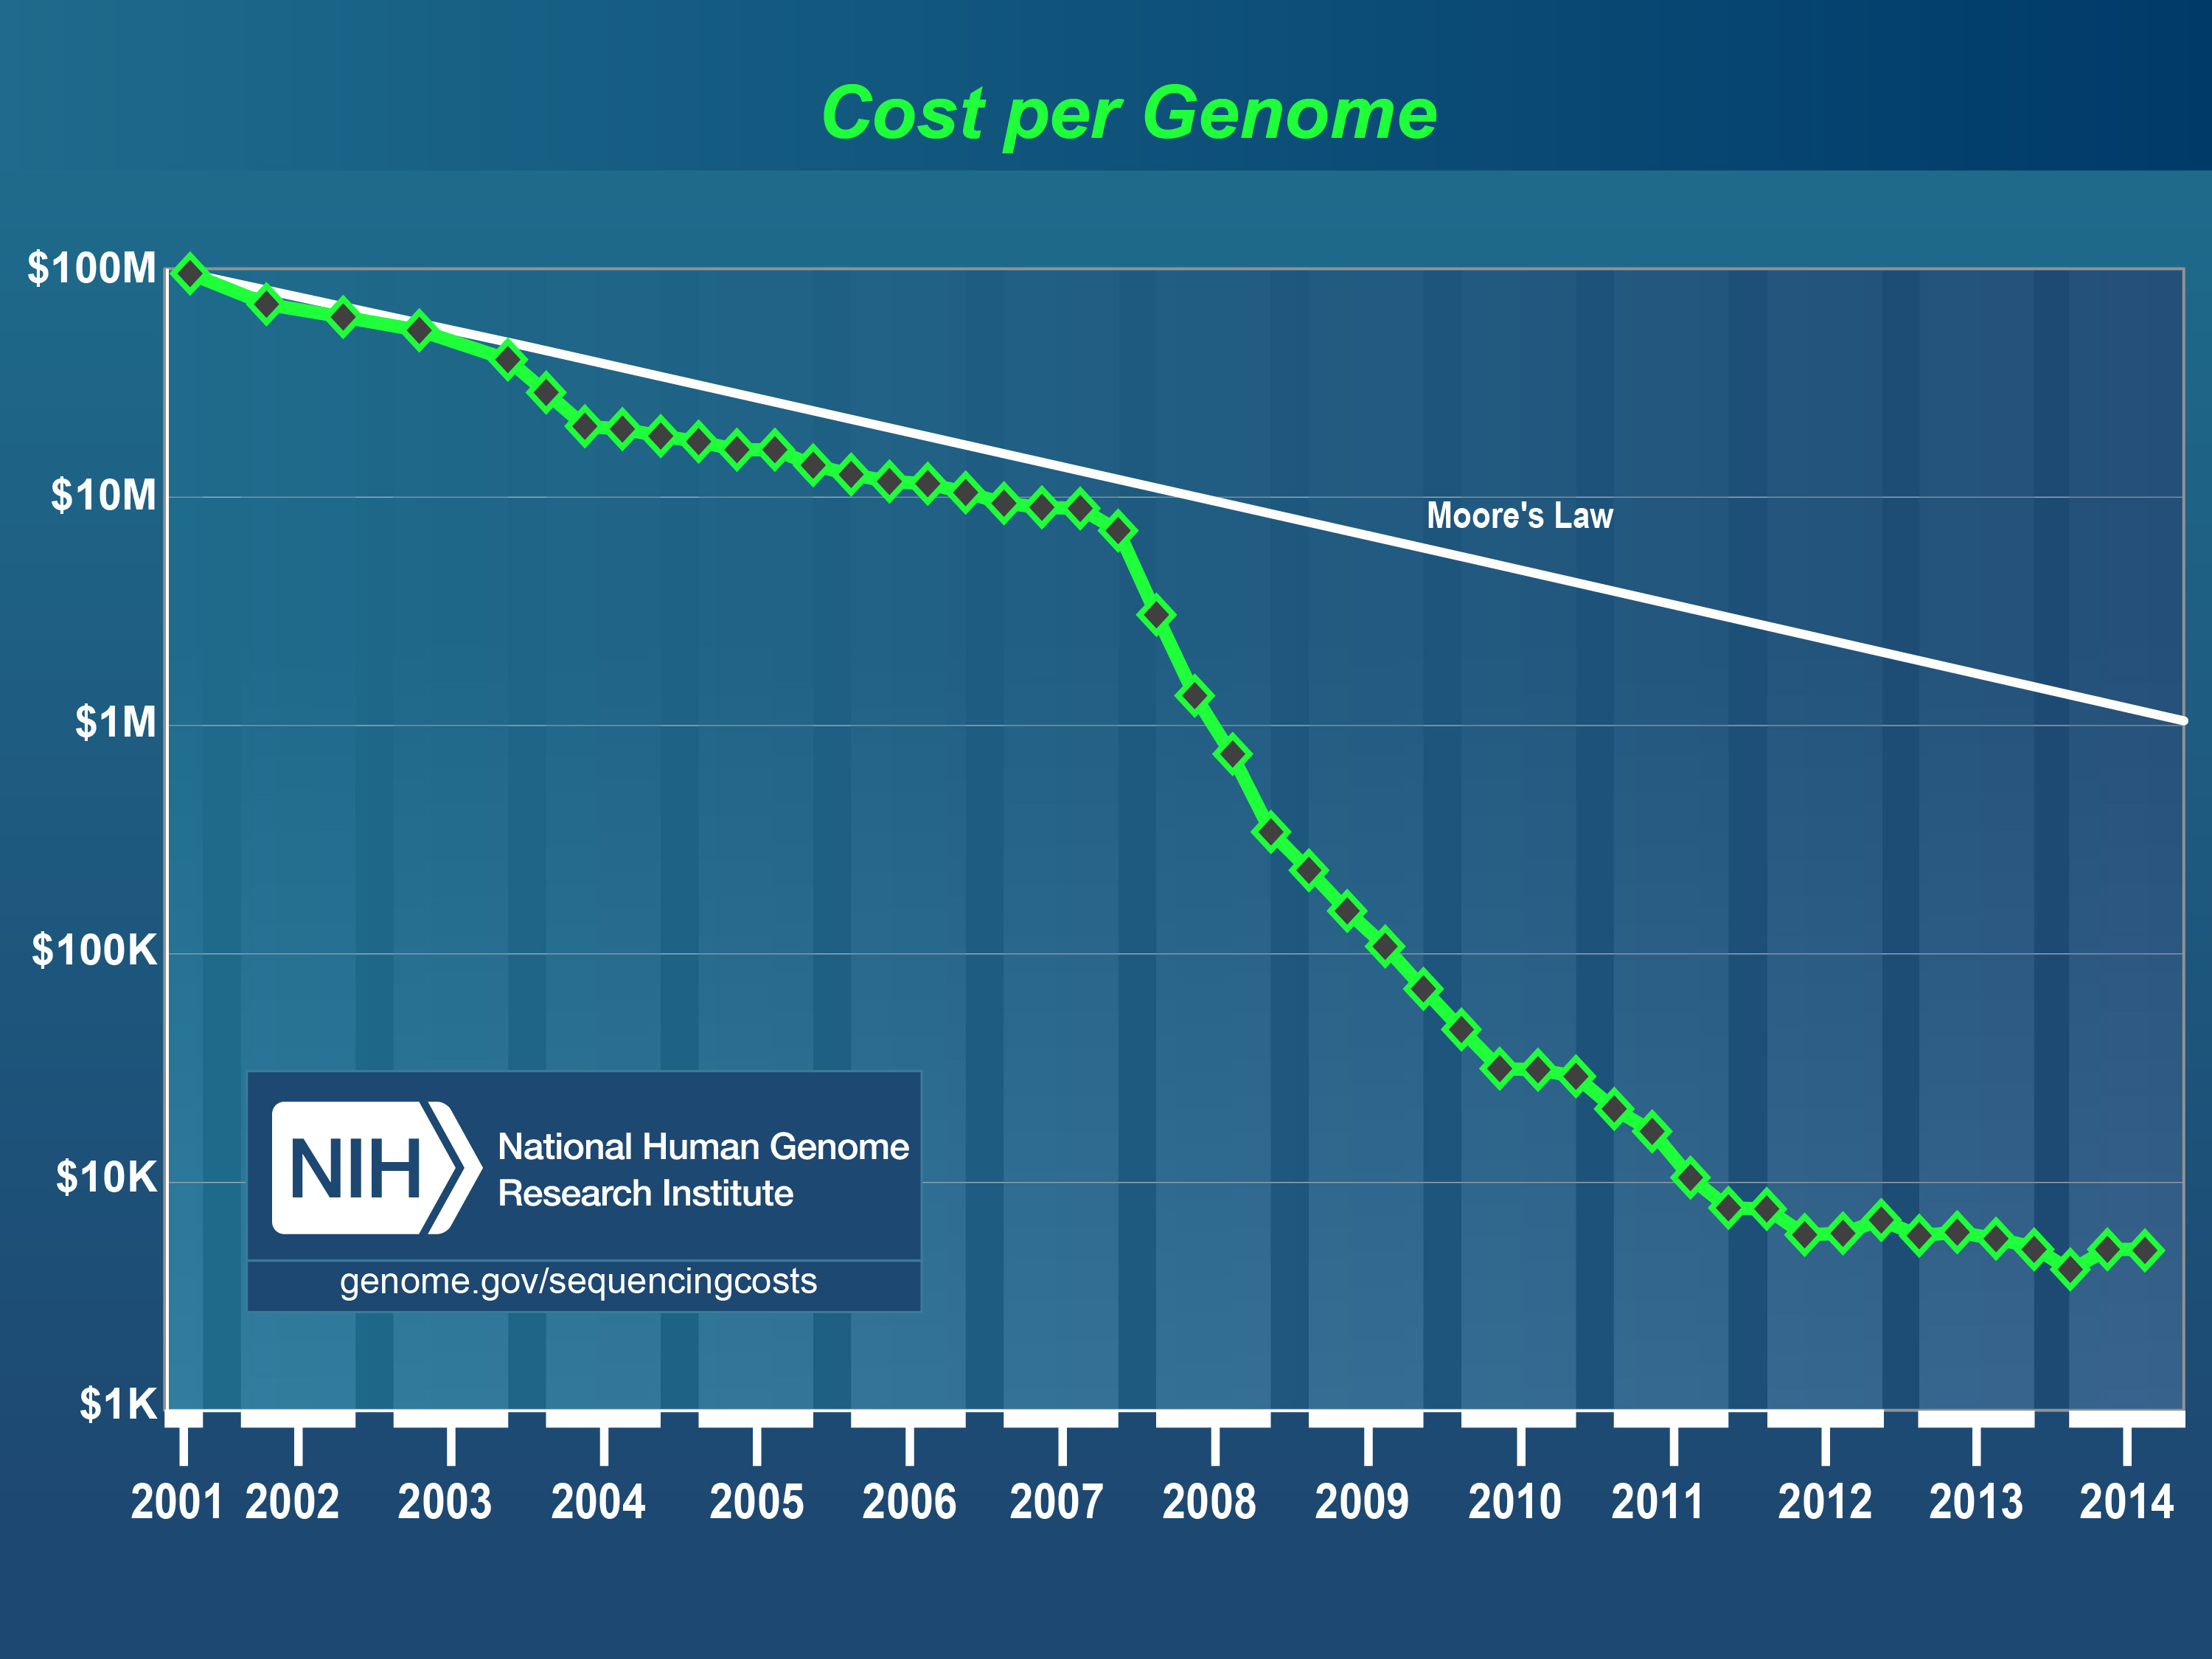
\includegraphics[width=\textwidth,height=\textheight,keepaspectratio]{cost_genome}
\caption{Evolutie van de prijs om een genoom te sequencen sinds 2001}
\label{sequencing_cost}
\end{figure}

\section{GEMINI}

Deze thesis bevat ook een case study over de opportuniteiten voor NoSQL-technologie\"en in de genoomanalysewereld. Op vraag van Janssens Pharmaceutica is het onderwerp hiervan de genoomanalysetool GEMINI (van GEnome MINIng): een software-framework voor flexibele analyse van genetische variaties in grote datasets van genomen, ontwikkeld aan de University of Utah \cite{10.1371/journal.pcbi.1003153}. GEMINI vertrekt daarbij van VCF (Variant Call Format) tekst-bestanden, laadt deze in in een database, voegt allerlei annotaties toe met bijkomende informatie van enkele vermaarde onderzoeksinstituten en biedt dan de mogelijkheid queries uit te voeren op deze databank. De huidige operationele versie van GEMINI draait op de eenvoudige SQL-databank SQLite, maar deze laat op gebied van schaalbaarheid en performantie te wensen over. De gewenste schaalbaarheid ligt in 2 dimensies: enerzijds het aantal genetische \textit{variants} in de dataset, d.w.z. stukken van genen zoals deze in het genoomsequencingproces waargenomen worden, en het aantal proefpersonen of \textit{samples} wier DNA in de dataset geanalyseerd wordt. Bij toenemend 
%TODO getal!
aantal samples of variants duurt zowel het inladen van de genoomdata in de databank voor als het query'en tijdens effectief gebruik te lang om gebruiksvriendelijk te zijn. Het inladen van de genoomdata uit VCF-files is, enigszins contra-intu\"itief, geen eenmalige of zeldzame operatie: de huidige productieversie van GEMINI laat niet toe om na het inladen nog samples of variants toe te voegen, met als gevolg dat bij elke iteratie van een genetisch of biologisch experiment die nieuwe informatie oplevert, de volledige dataset opnieuw ingeladen dient te worden. Ook het incrementeel kunnen toevoegen van variants en samples aan de gegevensset is dus een aandachtspunt bij het onderzoek naar mogelijke verbeteringen voor GEMINI.\\
Een eerste oplossing om de performantie te verhogen was om over te schakelen op PostgreSQL, en hiervan is intussen al met succes een eerste versie ge\"implementeerd. Het resultaat is een verhoging van de querysnelheden van 5 tot 20x, zonder verregaande optimalisaties. De verwachtingen zijn echter ook hier dat PostgreSQL op langere termijn niet zal kunnen schalen naar datasets van (honderd)duizenden genomen.\\
Naar de toekomst toe is het dus noodzakelijk uit kijken naar andere technologie\"en en types databanken om GEMINI ook bruikbaar te maken voor grootschaligere experimenten.




\chapter{Achtergrond databanken}
\label{cha2}

Sinds de jaren '70 zijn zogenaamde \textit{relational database management systems} (kortweg RDBMS) de voornaamste technologie voor de grootschalige opslag van gegevens. Ze zijn gestoeld op 2 belangrijke principes, namelijk het relationele datamodel \cite{codd1970relational} en de gestructureerde querytaal SEQUEL, beter gekend als SQL \cite{chamberlin1974sequel}. De architectuur van vele RDBMS is nog steeds gebaseerd op de eerste implementatie van een dergelijk systeem, namelijk het IBM onderzoeksproject System R \cite{blasgen1981system}, ook uit halverwege de jaren '70. System R is uiteraard ontworpen voor destijds relevante hardwarekarakteristieken en productvereisten: business data processing via een command line interface, en dit op computersystemen met trage processoren, kleine werk- en schijfgeheugens maar relatief grote bandbreedte tussen de schijfopslag en het werkgeheugen \cite{Stonebraker:2007:EAE:1325851.1325981}. Dit leidde tot een aantal architecturale features die nog steeds terug te vinden zijn in hedendaagse RDBMS:
\begin{itemize}
\item Disk-geori\"enteerde opslag- en indexstructuren
\item Multithreading om latency te verbergen
\item Concurrency-controlemechanismen op basis van locking
\item Log-gebaseerd herstel van fouten
\end{itemize} 
Ondanks gigantische technologische vooruitgang op gebied van hardware en sterk gediversifieerde gebruiksscenario's, is er sinds hun ontstaan 40 jaar geleden weinig drastisch veranderd aan het concept van de RDBMS en zijn deze systemen de werkpaarden van de industrie geworden op het vlak van dataopslag.\\

Beginnende in de jaren 2000 groeide in de IT-wereld dan ook het besef dat de rigide "one size fits all"-aanpak van RDBMS voor vele moderne toepassingen achterhaald dreigde te geraken. Met grote opkomende spelers uit de <eb-industrie zoals Google, Amazon en Facebook aan het roer leidde dit tot de opkomst van de NoSQL-beweging. NoSQL staat, in tegenstelling tot wat de naam doet vermoeden, voor "Not only SQL" en omvat een waaier van uiteenlopende alternatieve gegevensopslagsystemen die elk in bepaalde specifieke opzichten meerwaarde trachten te bieden ten opzichte van het klassieke relationele systemen. In tegenstelling tot de 'Zwitsers zakmes'-aanpak van RDMBS, leggen ze zich toe op zeer gespecialiseerde toepassingsdomeinen en proberen daarin relationele systemen te overtreffen. Vaak betekent dit dat NoSQL systemen vele voor hun doel onnodig geachte features van SQL systemen achterwege laten, of afzwakken. Een goed voorbeeld hiervan zijn de ACID-eigenschappen uit het relationele model die in vele NoSQL-systemen gereduceerd zijn tot zogenaamde BASE-eigenschappen (op het verschil tussen beide komt onderstaande sectie nog uitgebreid terug).

\section{Begrippen}

Deze sectie belicht de belangrijkste technische begrippen in verband met NoSQL-databanken en contrasteert waar nodig met gelijkaardige concepten in het klassieke traditionele model.

\paragraph{Consistentie}

Consistentie van database-transacties betekent dat transacties de databank in een consistente staat achterlaten: alle data die een applicatie kan zien, is een consistente snapshot van de databank \cite{ports2010transactional}. Traditionele RDBMS bieden vaak transacties met de zogenaamde ACID-eigenschappen \cite{haerder1983principles}:
\begin{itemize}
\item \textbf{Atomicity:} Elke transactie gebeurt ofwel volledig, ofwel helemaal niet.
\item \textbf{Consistency:} Elke transactie laat de databank in consistente staat achter.
\item \textbf{Isolation:} Elke transactie verloopt volledig ge\"isoleerd van elke andere transactie en be\"invloedt deze dus op geen enkele manier.
\item \textbf{Durability:} Eens voltrokken, blijft elke transactie duurzaam bewaard in de databank, ook in het geval van stroomonderbrekingen, crashes of fouten.
\end{itemize}

Zoals Eric Brewer stelde in zijn bekende CAP-theorema \cite{brewer2000towards}, is het in een gedistribueerd systeem niet eenvoudig zowel consistentie, availability als tolerantie voor partities te bereiken en zijn 2 van deze 3 eigenschappen het hoogst haalbare\footnote{Brewer kwam hier zelf 12 jaar later op terug, stellende dat mits goede omgang met partities het toch mogelijk is een trade-off van alle drie te bereiken \cite{brewer2012cap}.}.
Ook in NoSQL-systemen, die vaak gedistribueerd van aard zijn, is het garanderen van consistentie geen triviale opgave. Afhankelijk van de gehanteerde schrijfstrategie is het mogelijk dat verschillende knopen in het cluster verschillende versies van data zien, als updates nog niet in het volledige cluster doorgekomen zijn. Daarom is er het onderscheid tussen strikte en uiteindelijke ("\textit{eventual}") consistentie: strikte consistentie is de gekende vorm waarin updates onmiddellijk zichtbaar zijn op alle nodes in het cluster, en dus ook naar bovenliggende applicaties toe. In het geval van uiteindelijke consistentie garandeert het systeem enkel dat na verloop van tijd alle nodes in het cluster dezelfde, up-to-date versie van de data zullen zien. NoSQL-systemen bieden dan ook vaak de BASE-eigenschappen, een zwakkere versie van de ACID-garanties:
\begin{itemize}
\item \textbf{Basically available:} Het systeem is onder quasi alle omstandigheden beschikbaar.
\item \textbf{Soft state:} Het systeem verkeert niet altijd in een consistente staat
\item \textbf{Eventually consistent:} Na verloop van tijd zal het systeem in een gekende staat verkeren.
\end{itemize}

Vele NoSQL-systemen stellen de gebruiker echter niet voor een voldongen feit bij de keuze tussen strikte en uiteindelijke consistentie: dankzij zogenaamde \textit{quora} kan de gebruiker zelf configureren welke consistentie het systeem levert. Door lees- en schrijfquora in te stellen, kan de gebruiker tunen hoeveel replica's respectievelijk moeten returnen bij een schrijfopdracht, en het welslagen van een schrijfopdracht moeten bevestigen. Op deze manier kan de gebruiker zelf een trade-off maken tussen snel lezen, schrijven en de behaalde consistentie. Bovendien zal de gebruiker, wanneer de som van het lees- en schrijfquorum groter is dan de replicatiefactor van het cluster, steeds de meest recente versie van gegevens zien, wat hetzelfde betekent als onmiddellijke, strikte consistentie.

\section{NoSQL-klassen}

NoSQL databanken zijn er in verschillende soorten en kunnen op basis van hun datamodel in een aantal categorie\"en onderverdeeld worden:

\begin{itemize}
\item \textbf{Key-Value stores} Deze zijn vergelijkbaar met dictionaries en mappen unieke keys op values. Deze values zijn voor de databank volledig betekenisloze byte-arrays en de enige manier om ze op te vragen, is via de bijhoren key. Voor zeer eenvoudige toepassingen resulteert dit in hoge lees- en schrijf-throughput, maar meer geavanceerde features zoals indexing, queries, en het modelleren van relaties binnen de data zijn hierdoor niet mogelijk\cite{hecht2011nosql}\cite{grolinger2013data}.

\item \textbf{Columnar stores} Deze zijn gebaseerd op het datamodel dat Google's BigTable heeft ge\"introduceerd en slaan data op in een spaarse, gedistribueerde, persistente en multidimensionele gesorteerde map\cite{chang2008bigtable}. In het geval van BigTable zijn dit drie dimensies: row key, column key en een timestamp. Omdat ook hier het systeem de opgeslagen data niet interpreteert, is het modelleren van relaties niet op een effici\"ente manier mogelijk. Dit wordt overgelaten aan de bovenliggende applicatie\cite{hecht2011nosql}.

\item \textbf{Document stores} Deze bewaren data als key-value paren en encapsuleren deze in documenten. Values kunnen van een brede waaier aan types zijn, zoals geneste documenten, lijsten of scalars. De namen van attributen kunnen dynamisch gespecifieerd worden tijdens runtime en moeten geen vooraf vastgelegd schema volgen\cite{cattell2011scalable}. Dit is geschikt voor het modelleren van ingewikkelde datastructuren. Vele document stores gebruiken het JSON-bestandsformaa (of een daarvan afgeleide vorm). In tegenstelling tot columnar stores, zijn de waarden in documenten niet betekenisloos voor het document store systeem en het is dus mogelijk hier indexen op te defini\"eren en queries op uit te voeren\cite{hecht2011nosql}.

\item \textbf{Graph databases} Zoals de naam doet vermoeden, stammen deze uit grafentheorie en maken ze gebruik van grafen als datamodel. Ze zijn uitermate geschikt om sterk verweven data te beheren, van bronnen zoals sociale netwerken of location based services. Hiervoor doen ze beroep op effici\"ente mechanismen om grafen te doorlopen waar andere systemen kostelijke operaties als recursieve joins gebruiken\cite{hecht2011nosql}.

\end{itemize}

De term NewSQL slaat op een verzameling systemen die ambi\"eren het klassieke relationele datamodel te combineren met de schaalbaarheid, distributie en fouttolerantie van NoSQL systemn. Hoewel ze allen de gebruiker het relationele model en SQL-achtige query mogelijkheden bieden, verschillen NewSQL stores onderling grondig, afhankelijk van de onderliggende architectuur. Zo zijn er onder meer systemen die gebouwd zijn bovenop bestaande NoSQL databanken, en andere die alle data in main memory opslaan.\cite{grolinger2013data}



\chapter{GEMINI overzicht}
\label{cha3}

Zoals eerder vermeld is GEMINI een applicatie voor de flexibele analyse van genoomdata van populaties van menselijke individu\"en. Deze sectie gaat dieper in op de belangrijkste features en het onderliggende datamodel van GEMINI in zijn oorspronkelijke vorm.

\section{Datamodel}

GEMINI importeert genetische variants en genotypes van alle gesampelde individu\"en (ook 'samples') vanuit een VCF file in een relationele database.
Daarnaast kan extra informatie over de samples, zoals geslacht, phenotype en onderlinge verwantschappen, meegegeven worden in een PED-file (van pedigree) om latere analyse te vergemakkelijken.\\

Elke variant in een input VCF file wordt uitvoerig geannoteerd na automatische vergelijking met bestaande of door de gebruiker gedefinieerde genoom-annotatiebestanden. De geannoteerde variants vormen de rijen van de hoofdtabel van de database, de \texttt{variants}-tabel. Deze tabel bevat ook voor elke variant informatie over elke sample, zoals diens genotype, de kwaliteit en diepte van de meting voor de variant in kwestie. In de SQLite-versie van GEMINI wordt dit opgeslagen als een gecomprimeerde array per variant, 1 voor elke sample-eigenschap: zo is er een \texttt{gt\_type}-kolom met arrays met de genotypes, en een \texttt{gt\_depth}-kolom met arrays met de diepte van de meting van elke sample voor elke variant. Samen met de \texttt{samples}-tabel, die voor elke sample zaken als het geslacht, phenotype en familierelaties bijhoudt, ligt de \texttt{variants}-tabel aan de basis van de uitgebreide query-mogelijkheden die GEMINI biedt.\\

Daarnaast zijn er nog tabellen zoals de \texttt{variant\_impacts}- en \texttt{gene\_detailed}-tabellen die respectievelijk extra informatie over de variants en het menselijk genoom bevatten. Deze informatie komt in het eerste geval eveneens uit de annotatiebestanden, en in het tweede uit tekstbestanden met referentie-informatie over het menselijk genoom die GEMINI, indien gewenst mee inlaadt.\\
Ten laatste zijn er nog enkele kleine tabellen met meta-informatie, zoals de \texttt{resources}-tabel die de gebruikte annotatie-files bevat, en de \texttt{version}-tabel die bevat doorn welke versie van GEMINI de data ingeladen is.\\\\

Een belangrijke troef van GEMINI en z'n datamodel is de flexibiliteit die het laat naar de gebruiker. Zo kan de gebruiker zelfgedefinieerde annotatie-files gebruiken, en zelf kolommen toevoegen aan de PED-files met informatie over de samples. Deze extra informatie zal GEMINI automatisch in de resp. \texttt{variants}- en \texttt{samples}-tabel opnemen en kan de gebruiker later ook doorzoeken.

\begin{figure}[h]
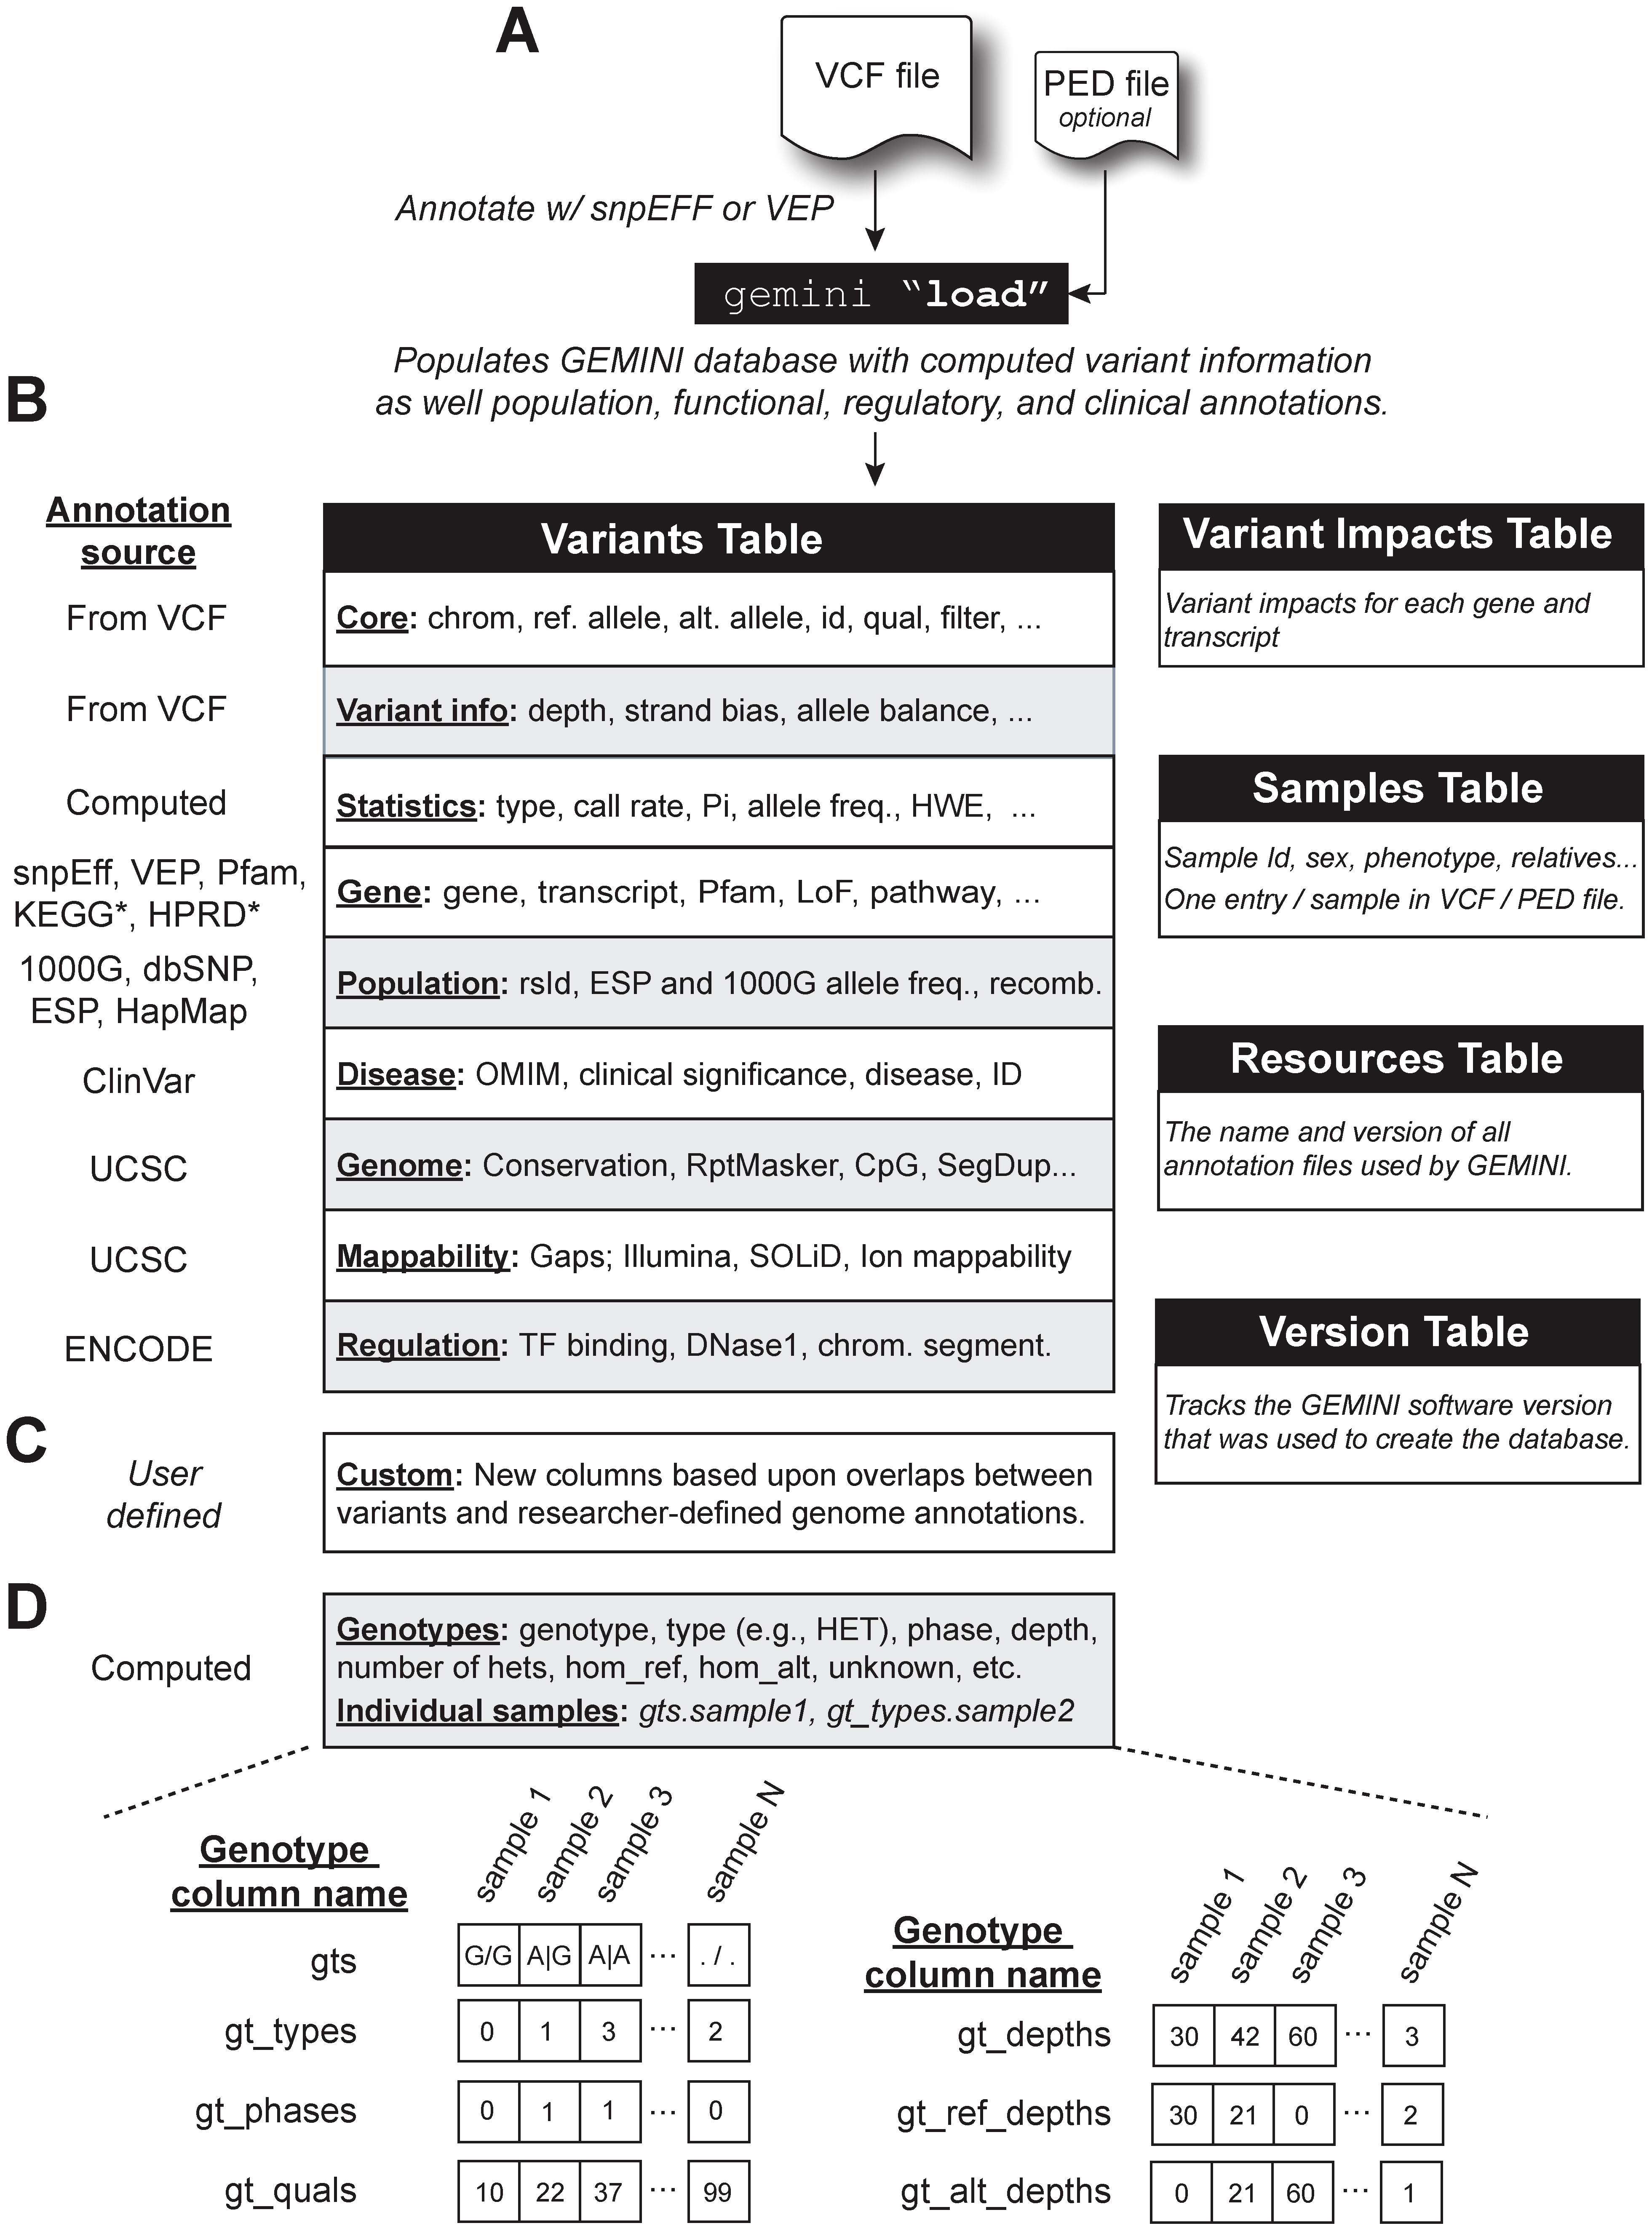
\includegraphics[scale=0.8]{gemini_schema}
\caption{Een overzicht van GEMINI's schema}
\label{gemini_schema_pic}
\end{figure}

\section{Inladen}
%TODO ref nr IPython dink
Het inladen van de data uit VCF-bestanden is een computationeel intensieve operatie, enerzijds omwille van de enorme grootte van deze bestanden, en anderzijds omdat in deze fase ook alle variants geannoteerd moeten worden. Om het proces te versnellen, biedt GEMINI de mogelijkheid het werk te paralleliseren door het VCF-bestand de comprimeren, op het bestaande bestand een index te defini\"eren en zo het werk te verdelen. Dit kan simpelweg over meerdere processoren binnen 1 computer zijn, maar via de IPython-interface ook over volledige clusters van computers.\\



\chapter{Datamodel Cassandra}
\label{cassandra_datamodel}

Het datamodel van Apache Cassandra vertoont enkele sterke verschillen met het relationele datamodel. Dit vereist enkele grondige aanpassingen aan het database schema van GEMINI. In deze sectie komen de belangrijkste eigenschappen van Cassandra aan bod, hun gevolgen voor de belangrijkste database-functionaliteiten, en de uitgevoerde aanpassingen aan het onderliggende schema van GEMINI ten op zichte van de SQLite implementatie.

\section{Datamodel Cassandra}

Zoals eerder vermeld bewaart Cassandra de cellen in een tabel als een 2 dimensionele map van enerzijds een per rij gedefinieerde primary key, en de naam van een kolom. De inhoud van cellen die niet in de primary key van een rij liggen, heeft voor Cassandra geen enkele betekenis.\\
Die primary key bestaat uit 2 delen: het eerste is de partition key, deze bestaat uit minstens 1 kolom en de waarde hiervan die via het consistent-hashing mechanisme bepaalt op welke knopen in het cluster de rij terechtkomt. Het tweede, optionele, deel is de clustering key, en bepaalt in welke volgorde rijen met dezelfde partition key op 1 node bewaard worden. Dit is standaard in oplopende volgorde.\\\\

%TODO: ALLOW FILTERING
Omdat het inspecteren van cellen indruist tegen de principes van Cassandra, zijn de query-mogelijkheden eerder beperkt: zonder het defini\"eren van indices is het in \texttt{WHERE}-clausules enkel mogelijk beperkingen op te leggen aan kolommen in de primary key, en dan nog zo dat de bedoelde rijen binnen 1 partitie liggen, en opeenvolgend opgeslagen zijn. Daarom moet er een gelijkheidsbeperking opgelegd worden aan de volledige partition key, en mogen er zowel gelijk- als ongelijkheidsbeperkingen opgelegd worden aan de kolommen in de clustering key, maar enkel op voorwaarde dat de voorgaande kolom in de clustering key ook met een gelijkheidsbeperking gespecifieerd is. Op deze manier kan Cassandra queries zeer snel uitvoeren door ze a.d.h.v. de hash van de partition key naar een juiste node te routeren, en vervolgens via de overige opgegeven kolommen de locatie van de juiste rijen te berekenen (die omwille van de clustering allemaal opelkaar volgend opgeslagen zijn). Dit gebeurt zonder de waarden van individuele cellen te bekijken, maar dus enkel door het berekenen van een simpele hashfunctie. Range-queries zijn dus enkel mogelijk op kolommen in de clustering key en het is niet mogelijk \texttt{!=}-beperkingen te gebruiken in \texttt{WHERE}-clausules. Bovendien laat Cassandra enkel toe beperkingen met elkaar te combineren via conjuncties, dus niet via \texttt{OR}- of \texttt{NOT}-operatoren. Een uitzondering op dit laatste is de \texttt{IN}-operator: op deze manier kan de gebruiker meegeven in welke set van waarden een bepaalde kolom moet liggen, maar dit is ook enkel mogelijk op de laatste kolom in de partition key of de laatste kolom in de clustering key (maar weer op voorwaarde dat de voorgaande kolommen reeds beperkt zijn).\\
Cassandra laat toe om indices op kolommen te defini\"eren, maar deze zijn niet bijzonder nuttig. Ze laten enkel gelijkheidsbeperkingen toe (dus geen range-queries) en bovendien raadt Datastax het gebruik van indices op kolommen met zowel een zeer lage als een zeer hoge kardinaliteit af, dit omdat in het eerste geval de index tabel zal bestaan uit zeer weinig zeer lange rijen voor elk van de ge\"indexeerde waarden en in het tweede geval Cassandra bij een query op de ge\"indexeerde kolom door zeer veel verscheidene waarden zal moeten zoeken om een klein aantal resultaten te vinden \cite{when_to_use_index}.

\section{Database schema GEMINI}
Zoals blijkt uit bovenstaande beschrijving van het datamodel van Cassandra, leent het systeem zich niet zomaar tot ad-hoc querying: het is niet mogelijk op een performante manier zomaar aan willekeurige kolommen in een tabel voorwaarden op te leggen en deze voorwaarden met elkaar te combineren. Dit betekent dat bij het ontwerpen van het database schema al rekening gehouden moet worden met de queries die achteraf op de data mogelijk moeten zijn. Omdat het soort queries dat een tabel ondersteunt sterk samenhangt met de keuze van de primary key van de tabel en GEMINI meerdere, uiteenlopende soorten queries op elke tabel vereist, zal dit onvermijdelijk leiden tot duplicatie van data.\\\\

Het belangrijkste vraagstuk is hoe de genotype-kolommen uit het oorspronkelijke relationele model in Cassandra op te slaan. Hier zijn enkele opties voor:

\begin{itemize}

\item[Collection columns] Cassandra biedt zogenaamde collection types, zoals sets, lists of maps. Dit is vergelijkbaar met de bestaande implementatie in SQLite (buiten dat ze in Cassandra niet als binary blobs bewaard worden). Het nadeel is echter dat deze collections niet meer dan 65536 ($2^{16}$) entries kunnen bevatten, wat het hele nut van de migratie naar Cassandra zou ondermijnen.

\item[Super-\texttt{variants}-tabel] Een andere mogelijkheid is de \texttt{variants}-tabel uit te breiden met een kolom voor elke genotype-eigenschap van elke sample. Deze aanpak heeft als voornaamste voordeel dat de kolommen met genotype-eigenschappen van specifieke samples zonder omwegen uit de \texttt{variants}-tabel gehaald kunnen worden. Dit is vooral van belang voor de in (\ref{gemini_beschrijving}) beschreven sample-filters. Bovendien kan Cassandra tot 2 miljard cellen opslaan op 1 partitie, dus vormt het grote aantal kolommen dat dit model met zich meebrengt, geen probleem.\\
Het nadeel is echter dat het onmogelijk is ad-hoc queries te defini\"eren op genotypes van willekeurige eigenschappen zonder het gebruik van secundaire indices. Elke query die in een \texttt{WHERE}-clausule andere kolommen of samples betrekt, vereist om de hierboven beschreven redenen een andere keuze van de primary key om effici\"ent de juiste rijen te kunnen opzoeken.

\begin{table}[!htbp]
\begin{tabular}{@{}|l|l|l|l|l|l|l|l|l|l|@{}}
\toprule
variant\_id & ref & alt & \ldots & gt\_type\_bob & gt\_type\_bruce & \ldots & gt\_depth\_bob & gt\_depth\_bruce & \ldots \\ \bottomrule
\end{tabular}
\end{table}


\end{itemize}
 

\bibliographystyle{abbrv}
\bibliography{biblio}
\end{document}